\paragraph{IUP04 Visualizar lista de comentarios} \hspace{1cm}\\ 
\label{pant:IUP04} 

\textbf{\textcolor[rgb]{0, 0, 0.545098}{Objetivo}}\\
Esta pantalla de uso brinda al Practicante la posibilidad de visualizar los comentarios que el Entrenador ha registrado sobre su desempeño en la realización de cada una de sus rutinas.\\

\textbf{\textcolor[rgb]{0, 0, 0.545098}{Diseño}}\\
En la figura \ref{fig:IUP04} se muestra la pantalla \nameref{fig:IUP04}, la cual muestra al Practicante las rutinas realizadas, el desempeño general obtenido y el comentario correspondiente.\\

En la parte inferior derecha se encuentra el botón Regresar, el cual corresponde a regresar al menú principal.

\begin{figure}[H]
	\centering
		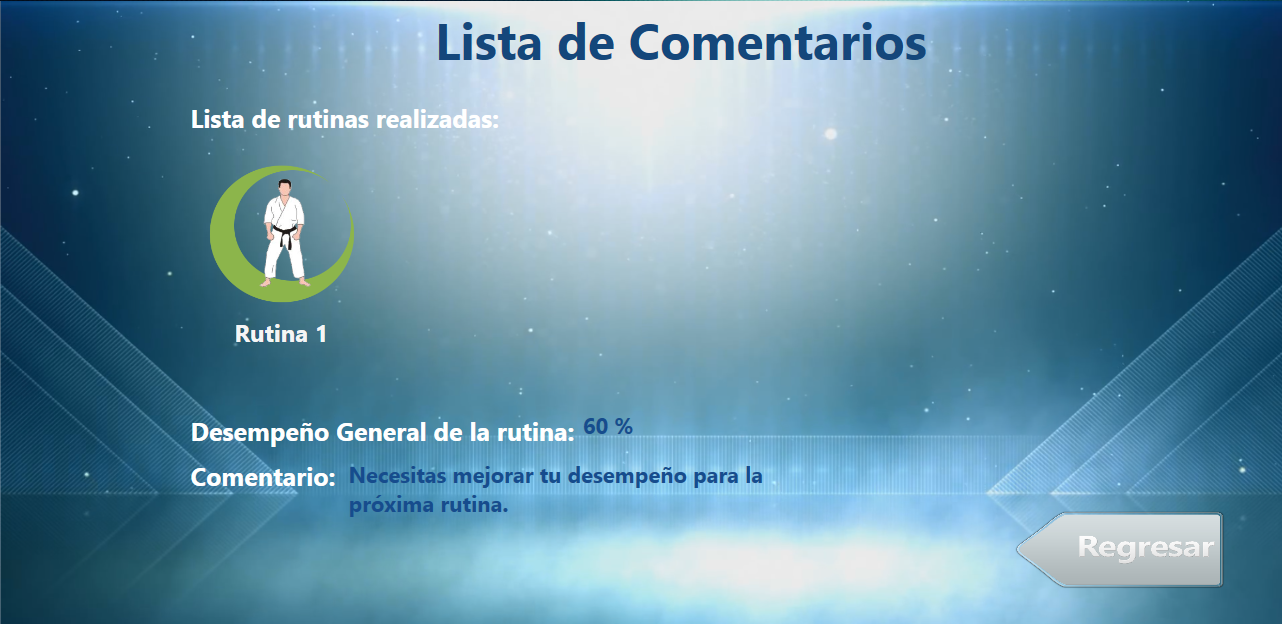
\includegraphics[scale=0.5]{./Figuras/Pantallas/IUP04Visualizar_lista_de_comentarios}
	\caption{IUP04 Visualizar lista de comentarios}
	\label{fig:IUP04}
\end{figure}

\textbf{\textcolor[rgb]{0, 0, 0.545098}{Comandos}}
\begin{itemize}
	\item \textbf{\textcolor[rgb]{0, 0, 0.545098}{Regresar:}} Regresa al menú principal \nameref{menu:MP01}.
\end{itemize}
\vspace{1em}

\textbf{\textcolor[rgb]{0, 0, 0.545098}{Mensajes}}\\

\textbf{\nameref{msj:MSG24}}: Se muestra en el menú principal \nameref{menu:MP01} cuando debido a un error de conexión no se muestren los elementos de forma correcta.\\

\clearpage